% Auto-generated by 04_additional_analysis.R — do not edit
% y > 0: Underreacts  |  y < 0: Overreacts
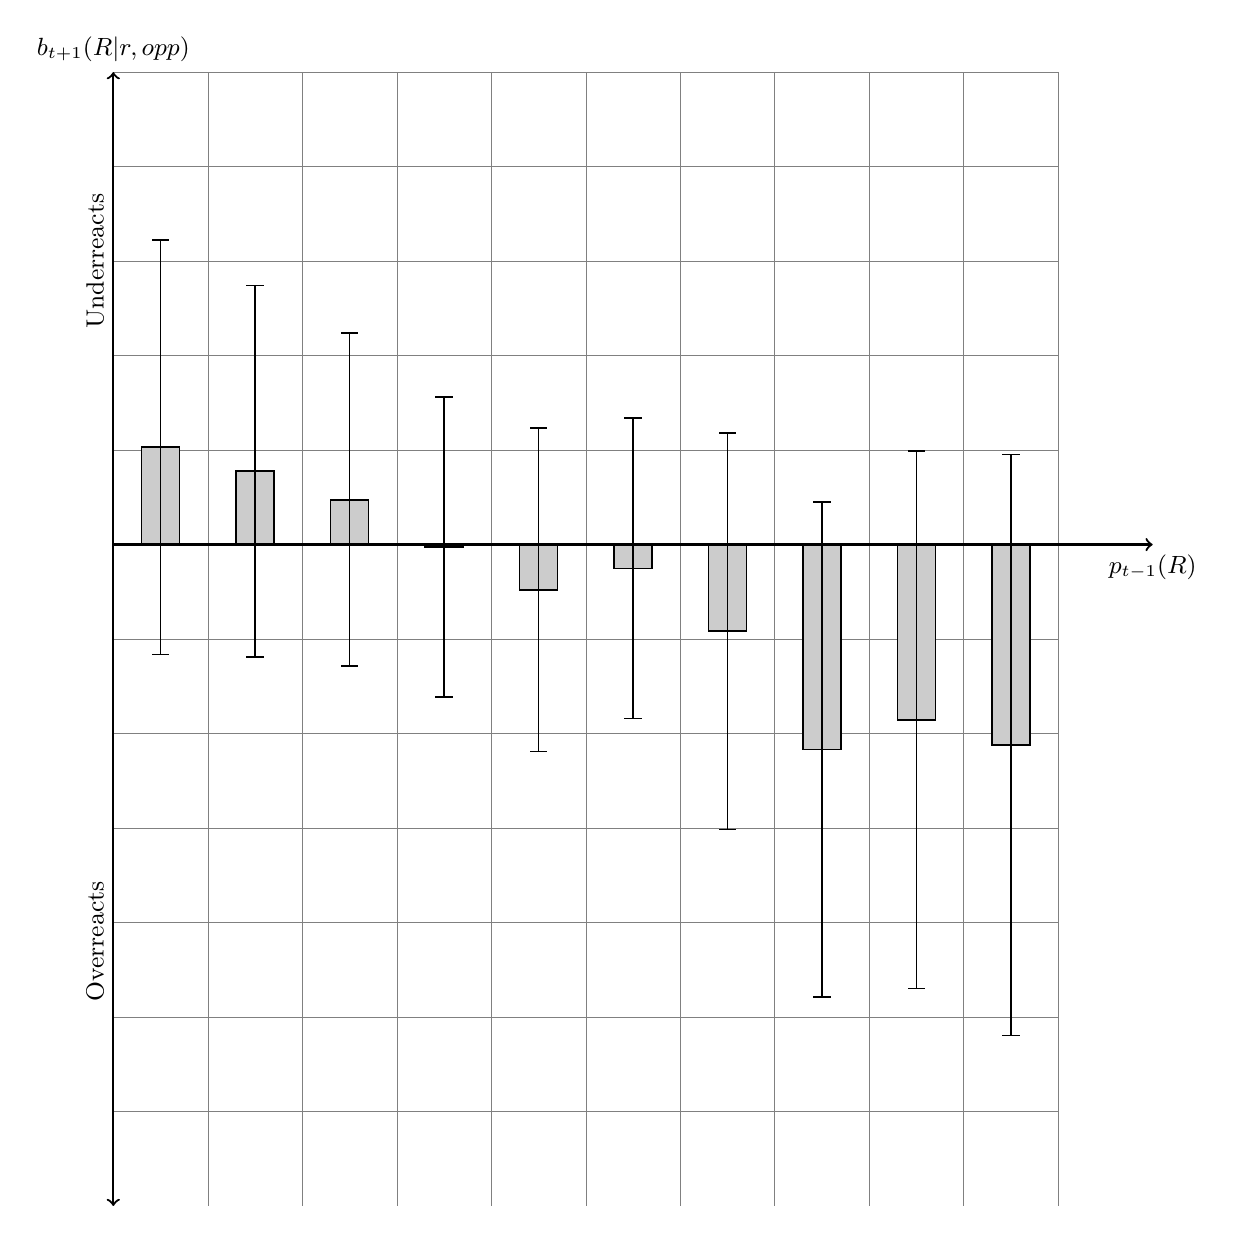
\begin{tikzpicture}[scale=12]
\draw[help lines,step=0.1] (0,-0.7) grid (1,0.5);
\filldraw[opaque,white!80!black] (0.03,0) rectangle (0.07,0.1031);
\draw[line width=0.6] (0.03,0) rectangle (0.07,0.1031);
\draw[line width=0.6,|-|] (0.05,-0.1173) -- (0.05,0.3235);
\filldraw[opaque,white!80!black] (0.13,0) rectangle (0.17,0.0777);
\draw[line width=0.6] (0.13,0) rectangle (0.17,0.0777);
\draw[line width=0.6,|-|] (0.15,-0.1198) -- (0.15,0.2752);
\filldraw[opaque,white!80!black] (0.23,0) rectangle (0.27,0.0475);
\draw[line width=0.6] (0.23,0) rectangle (0.27,0.0475);
\draw[line width=0.6,|-|] (0.25,-0.1296) -- (0.25,0.2245);
\filldraw[opaque,white!80!black] (0.33,0) rectangle (0.37,-0.0025);
\draw[line width=0.6] (0.33,0) rectangle (0.37,-0.0025);
\draw[line width=0.6,|-|] (0.35,-0.1619) -- (0.35,0.1569);
\filldraw[opaque,white!80!black] (0.43,0) rectangle (0.47,-0.0478);
\draw[line width=0.6] (0.43,0) rectangle (0.47,-0.0478);
\draw[line width=0.6,|-|] (0.45,-0.2199) -- (0.45,0.1242);
\filldraw[opaque,white!80!black] (0.53,0) rectangle (0.57,-0.0252);
\draw[line width=0.6] (0.53,0) rectangle (0.57,-0.0252);
\draw[line width=0.6,|-|] (0.55,-0.1851) -- (0.55,0.1346);
\filldraw[opaque,white!80!black] (0.63,0) rectangle (0.67,-0.0917);
\draw[line width=0.6] (0.63,0) rectangle (0.67,-0.0917);
\draw[line width=0.6,|-|] (0.65,-0.3024) -- (0.65,0.1190);
\filldraw[opaque,white!80!black] (0.73,0) rectangle (0.77,-0.2170);
\draw[line width=0.6] (0.73,0) rectangle (0.77,-0.2170);
\draw[line width=0.6,|-|] (0.75,-0.4797) -- (0.75,0.0457);
\filldraw[opaque,white!80!black] (0.83,0) rectangle (0.87,-0.1855);
\draw[line width=0.6] (0.83,0) rectangle (0.87,-0.1855);
\draw[line width=0.6,|-|] (0.85,-0.4707) -- (0.85,0.0996);
\filldraw[opaque,white!80!black] (0.93,0) rectangle (0.97,-0.2121);
\draw[line width=0.6] (0.93,0) rectangle (0.97,-0.2121);
\draw[line width=0.6,|-|] (0.95,-0.5204) -- (0.95,0.0962);
\draw[line width=0.8,->]  (0,0) -- (1.1,0) node[below] {\small{$p_{t-1}(R)$}};
\draw[line width=0.8,<->] (0,-0.7) -- (0,0.5) node[above] {\small{$b_{t+1}(R|r,\text{opp})$}};
\draw (0,0.30) node[above,rotate=90] {\small{Underreacts}};
\draw (0,-0.42) node[above,rotate=90] {\small{Overreacts}};
% ADD THEORY CURVE BELOW IF NEEDED:
% \draw[red,line width=1.2,domain=0.01:0.99] plot(\x,{...});
\end{tikzpicture}
